%%This is a very basic article template.
%%There is just one section and two subsections.
\documentclass[conference]{ieeeconf}

\IEEEoverridecommandlockouts 
\overrideIEEEmargins

\usepackage{graphics} % for pdf, bitmapped graphics files
\usepackage{epsfig} % for postscript graphics files 
\usepackage{multirow}
\usepackage{graphicx}
\usepackage{amsmath} 

\begin{document}


\title{Path towards a Fairness (QoS) control within the DSA Project}

\author{Andres Mora and Tomohiro Miyasaka}
\date{} % to elminate the date

\maketitle

\section{Introduction: The DSA approach}
The Dynamic Spectrum Access is a novel method to improve the performance of radio wave based communication systems, such as wireless local area network (WLAN) and Bluetooth.
This approach works in the 2.4[GHz] band (2400$\sim$2484 [MHz]), using methods such as the Fast Fourier transform (FFT), the power spectrum of the radio waves can be calculated.
DSA should be able to identify the different types of radio frequencies that may be present in the 2.4[GHz] band.
In this band, WLAN, Bluetooth, microwave ovens and other devices may operate creating interference between each other's signal.
DSA will address the interference that these devices induce into each other by identifying what type of device is transmitting over the above mentioned band, restricting the access of a given device to a selected frequency and therefore controlling and improving the throughput of the overall network.

The fairness control is composed of three main components:
\begin{enumerate}
  \item Sensing Strategy
  \item Communication Simulator to test our DSA approach (Design Traffic Model for General Radio Systems)
  \item Fairness Control
\end{enumerate}

In the following sections each of these components are further explained and the expected time to complete each of them is proposed.

This document shows a summary of the steps towards designing a ``fairness control'' or quality of service (QoS) that defines the DSA approach and the initial experiments, methodology and results from these initial experiments.
It is the first stage of the DSA project where robotics (and in particular mobile social robots) may become a feasible application.
For the networked robotics community, DSA may work as a backup protocol in the event of a problem with the current WLAN protocols for traffic control.
In this way, if several robots and operators are connected to the same network, DSA would help directing the traffic of the network in an appropiate manner.

\begin{figure}[htp] 
\centering
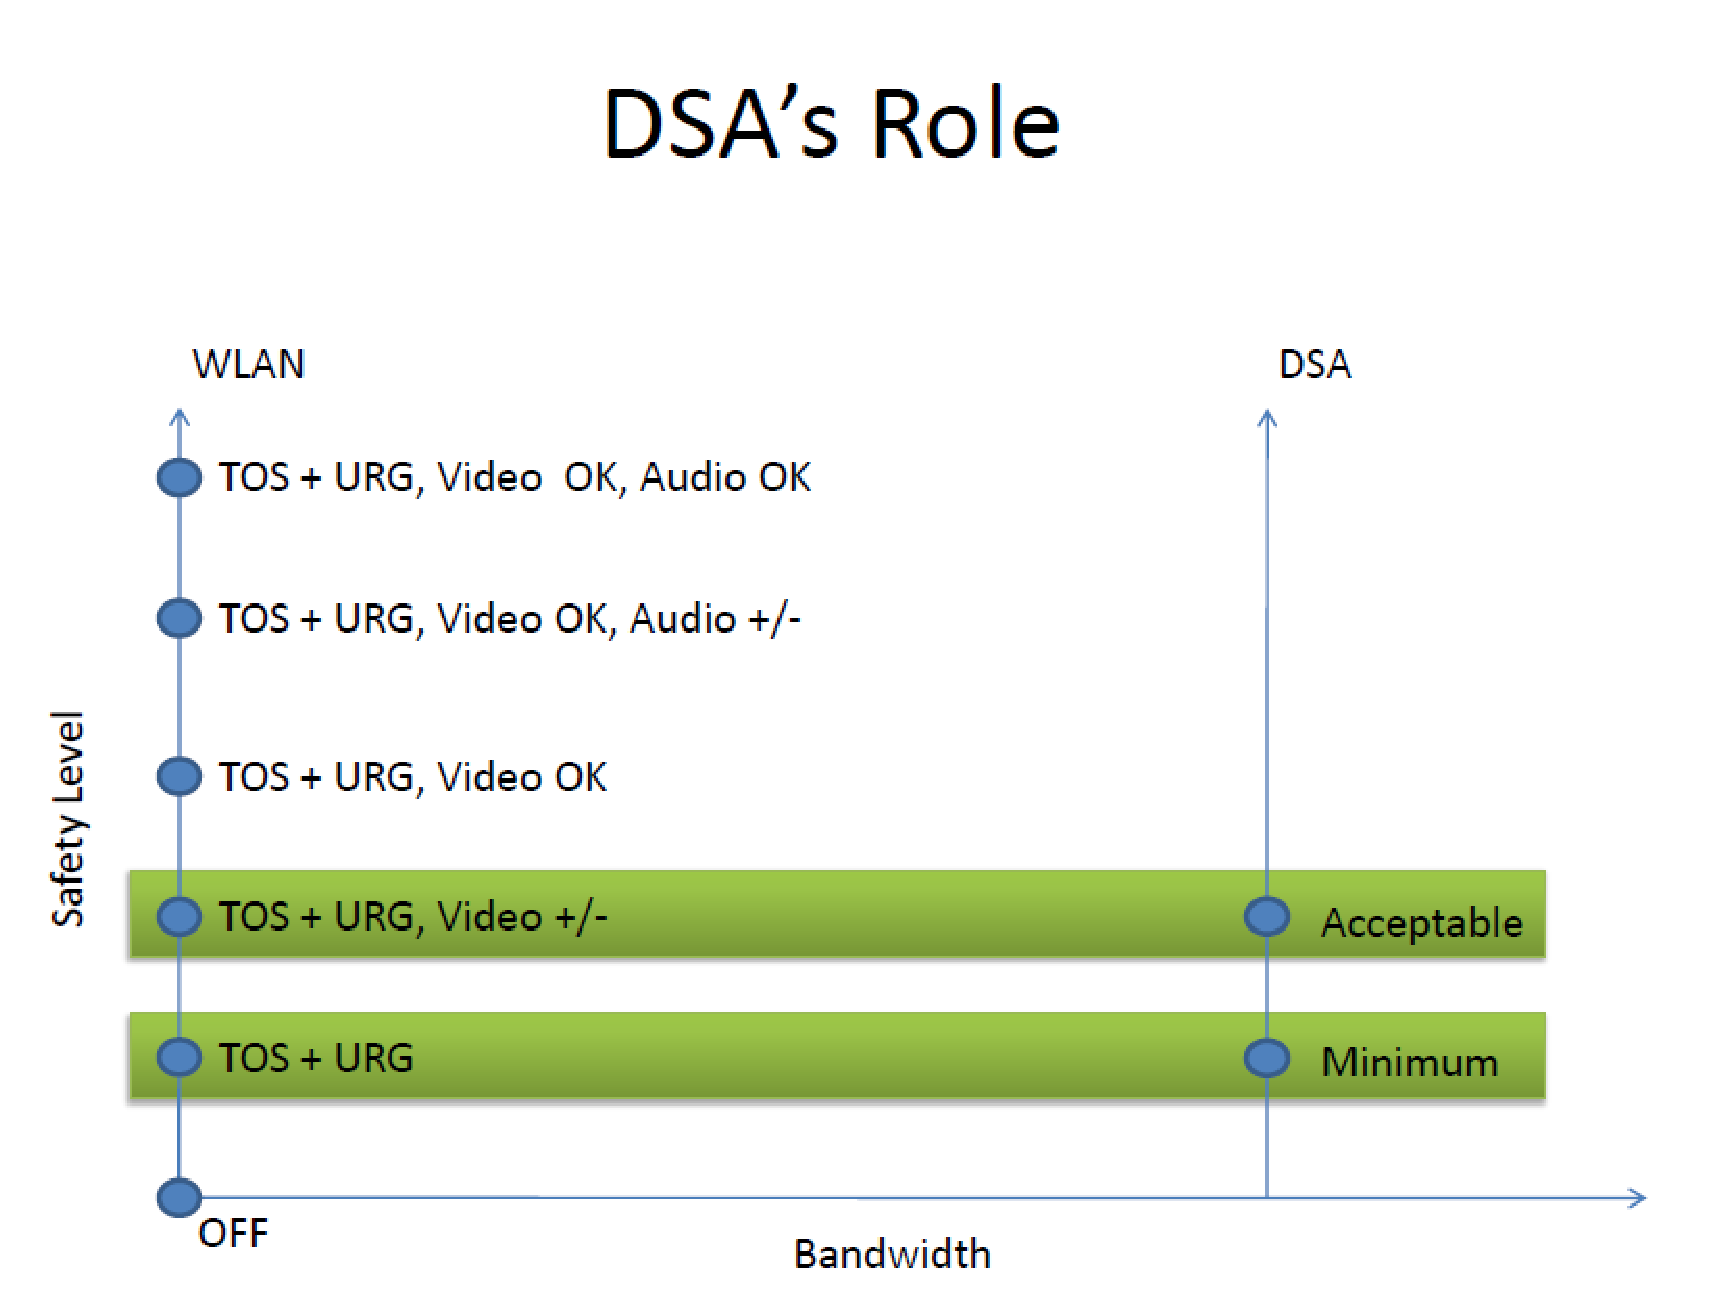
\includegraphics[width=1\columnwidth, scale=0.6]{dsaRole}
\caption{DSA may work as a backup protocol in the event of a problem with the current WLAN protocols for traffic control.}
\label{fig:dsaRole}
\end{figure}

\section{Sensing Strategy}
\label{sec:sensing}
This sensing strategy is focused on determining if there is an available interval within other wireless system's signals.
One can determine that if in a given frequency the value of its signal power spectrum is lower than a known threshold this frequency will not be used.
There are various problems with this approach.
One of them is that the power spectrum of a signal has a directly proportional relationship with the distance from its closest access point (AP).
Thus, a user may be sending/receiving data at a lower power level and this level may be ``sensed'' as below of the established threshold.

Another problem is that a WLAN may have transmitted a data frame will wait for to receive an acknowledgement (ACK) from its receiving party.
As part of the WLAN communication standard, the interval the transmitter (AP) waits after sending the data frame and the ACK is always 10[$\mu$sec], this is called the ``short interframe space'' or S-IFS.
If the transmitter does not prepare to listen to the ACK it may miss it.
In addition, if during the S-IFS interval period another WLAN signal is introduced or is present, it may cause an interference in the original signal.

It should be noticed that a simple approach as not using a given frequency because of its low power spectrum should be avoided since the S-IFS will not be able to be used.

A number of steps to accomplish this sensing strategy are shown as follows:

\begin{enumerate}
  \item Is it WLAN/BT/Microwave oven? 
  \begin{enumerate}
    \item What method should be used for this? 
    \item Type of packet 
  \end{enumerate}
  \item Is this an interval? 
  \begin{enumerate}
    \item What type of interval? 
    \item Output: Use or don't use this frequency's channel
  \end{enumerate}
\end{enumerate}

\section{Fairness Control}
\label{sec:fairness}
In a given location, a network may consist of WLAN and/or BT connections.
A typical example may be that of a WLAN connection being interfered due to the introduction of a BT connection and viceversa.
However in such case, if we can open an interval between a WLAN connection's packet and packet both the WLAN and the BT connection would be possible.
The problem is administering these intervals such that the WLAN allows the BT connection's packet to be present without causing interference to the original WLAN connection.

DSA aims to administer these intervals through a number of policies that consider the constraints of the WLAN, BT and other devices' connections within the same location.
Some of these constraints and the proposed policies are listed below.

\begin{enumerate}
  \item Policy definition 
\end{enumerate}

\begin{enumerate}
  \item Communication System's Constraints 
  \begin{enumerate}
    \item Signal's power 
    \item Signal's packet interval 
    \item BT automatically moves from one channel to the other fast and randomly
    \item WLAN has fixed channels 
  \end{enumerate}
\end{enumerate}

\section{Communication's Simulator}
\label{sec:simulator}
In order to test the components presented in Sections \ref{sec:sensing} and \ref{sec:fairness}, a simulator is required.
This simulator will be able to give a realistic representation of the communication between AP and wireless users.
The most important issue here is the design of a ``human behavior'' model that accurately represents people's usage of the network.

\begin{enumerate}
  \item Simulate one WLAN connection
  \begin{enumerate}
    \item Define AP (Server)
    \begin{enumerate} 
      \item IP's protocol
      \item TCP/UDP's protocol
      \item Application protocol 
      \item Server behavior based on a human's connection model
    \end{enumerate} 
    \item Define Wireless User 
    \begin{enumerate}
      \item IP's protocol
      \item TCP/UDP's protocol 
      \item Application protocol
      \item Human behavior model (How can this be defined? It is a ``non-stationary deterministic process'')
    \end{enumerate}
  \end{enumerate}
  \item Simulate multiple WLAN connections
  \item Integration of the sensing strategy presented in Section \ref{sec:sensing}.
\end{enumerate}

\begin{figure*}[t]
\centering
\begin{tabular}{@{}cc@{}}
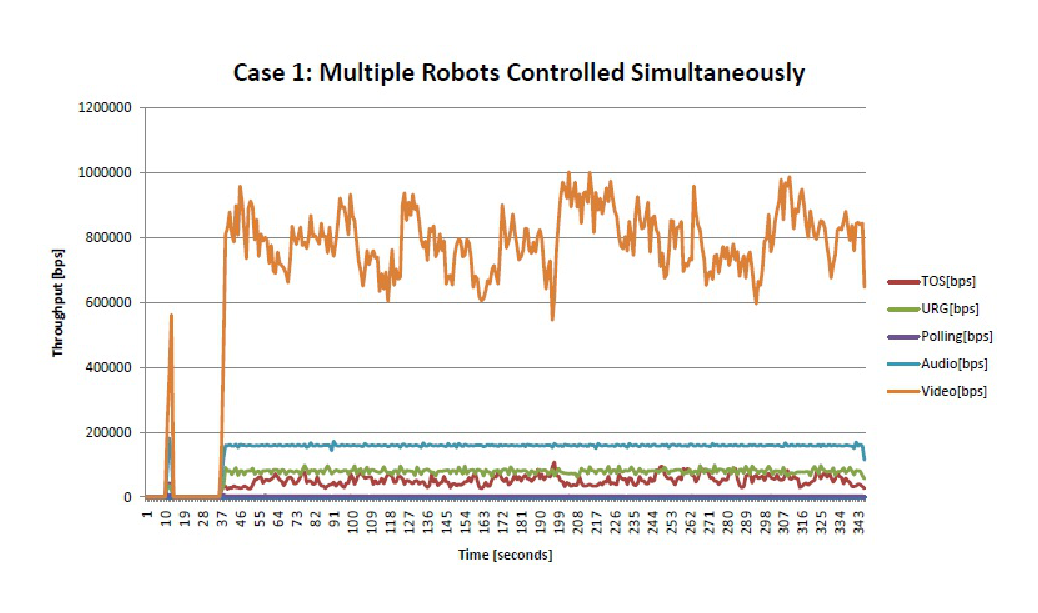
\includegraphics[width=\columnwidth]{multipleRobots} &
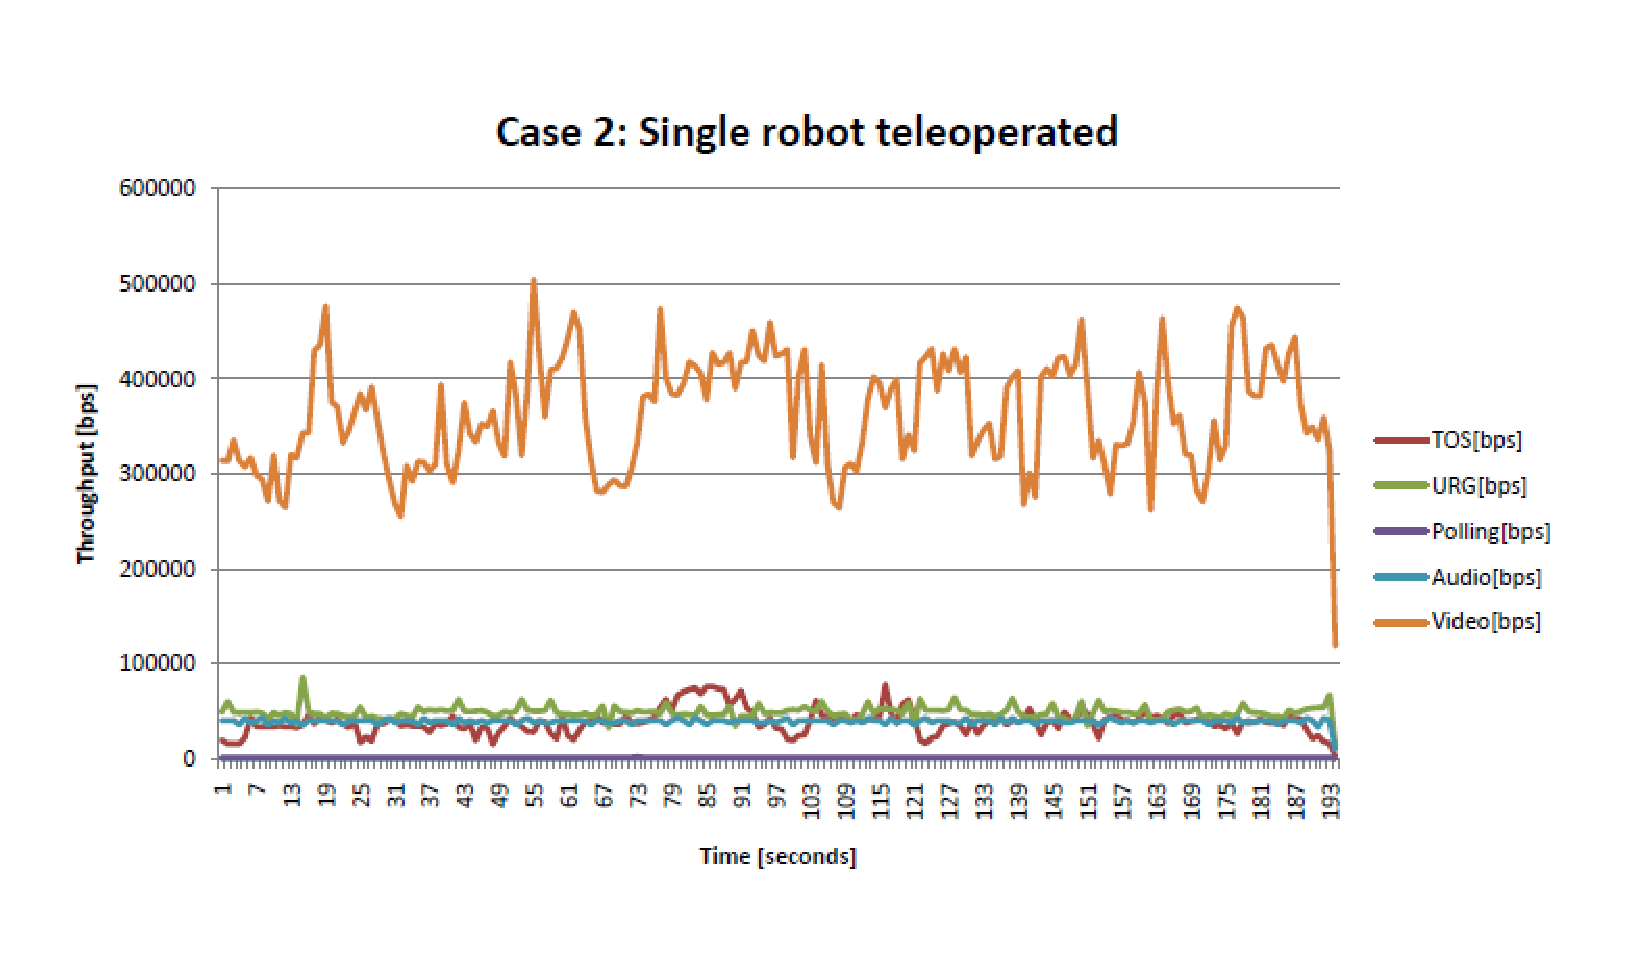
\includegraphics[width=\columnwidth]{singleRobot}\\
a) Multiple robots (Robovie-22 \& Robovie-Cart) &
b) Single robot (Robovie-Cart)\\
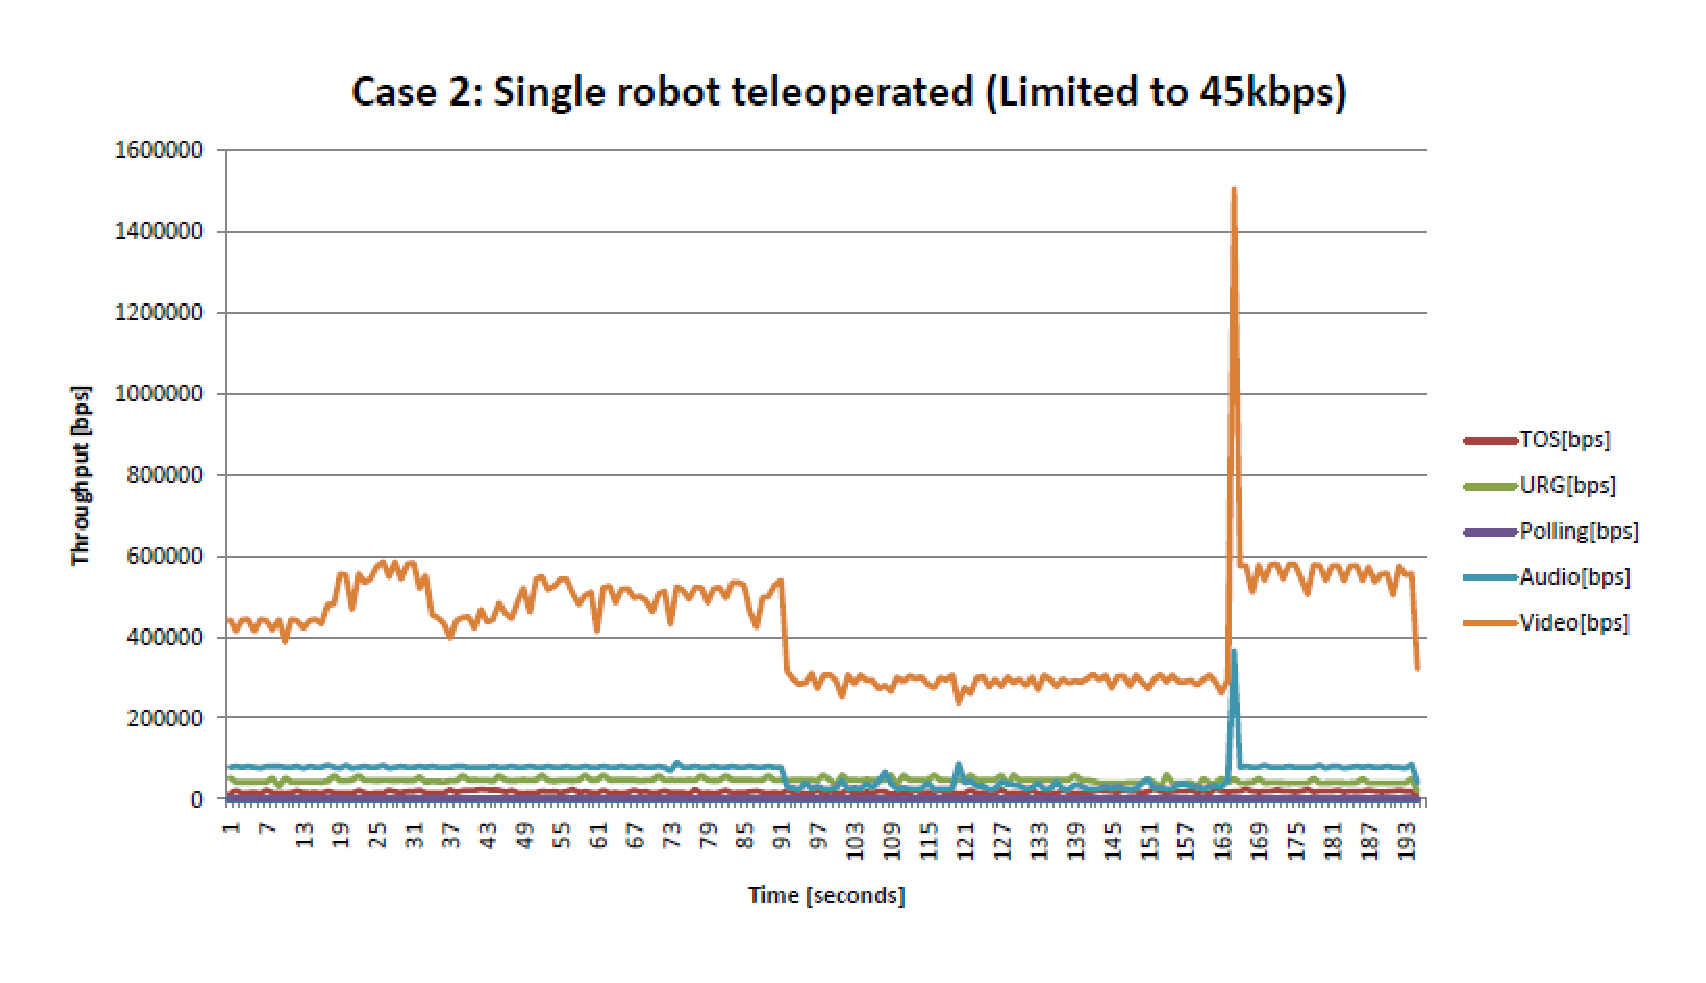
\includegraphics[width=\columnwidth]{singleRobot45K} &
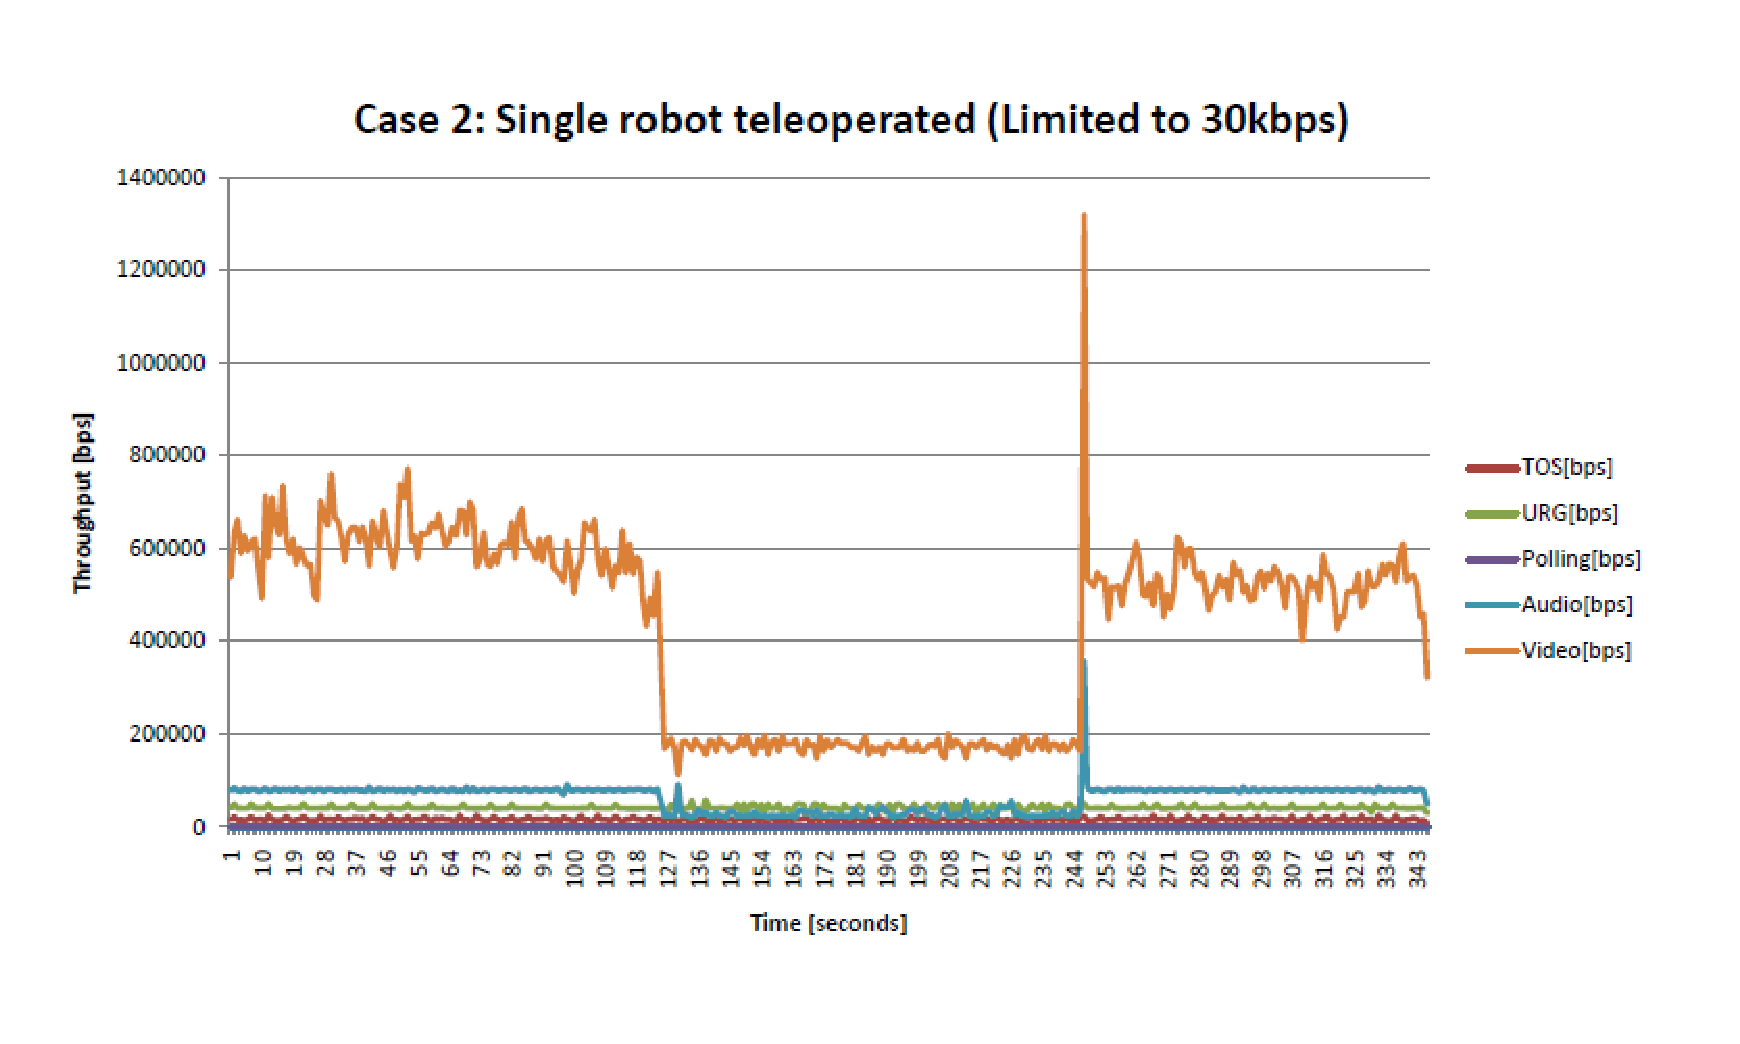
\includegraphics[width=\columnwidth]{singleRobot30K}\\
c) Network traffic limited to 45kbps &
d) Network traffic limited to 30kbps
\end{tabular}
\caption{{\Large Network traffic data obtained under different conditions.}}
\label{fig:expResults}
\end{figure*}

\section{Initial Experiments}
In order to understand which are the minimum requirements in terms of bandwidth consumption and traffic for a networked team of mobile social robots a set of initial experiments were carried out.

These experiments were intended to find the values at which one operator cannot manipulate a single or multiple mobile social robots at a time.
The robots used to carried out the experiments were Robovie-22 and Robovie-Cart.

Two sets of experiments were performed: 
\begin{itemize}
  \item [a)] Multiple robots: a single-operator-two-robots approach was used. 
  The operator simultaneously controlled two robots: Robovie-Cart and Robovie-22 using 3D-MRC.
  In this case, the operator used the On-board Human Tracker (OBHT) on Robovie-Cart to automatically follow the customer and manually controlled Robovie-22 to interact with the customer at the same time using gestures and text-speech conversation. 
  
  \item [b)] Single robot: a single-operator-one-robot approach was used. 
  The operator used the 3D version of Multirobot Controller (3D-MRC) to control a single robot, Robovie-Cart.
  In this case, the operator manually followed the customer and responded to questions.
  
  \item [c)] Single robot limited to 45kbps: same setup as in ``b)'' but in this case the throughput was limited to 45kbps.
  
  \item [d)] Single robot limited to 30kbps: same setup as in ``c)'' but in this case the throughput was limited to 30kbps.
\end{itemize}

Understanding these minimum required throughput values would allow DSA to know which is the minimum amount of throughput that it should provide to the robot being controlled at the moment. 
Figure \ref{fig:dsaRole} presents the role of DSA as a backup in case the allocation of bandwidth provided by standard WLAN protocols do not work. 

\section{Methodology}
The software used to measure the traffic of the packages on the network between the robot(s) and the operator was WireShark (www.wireshark.org). 
This software obtains all the raw traffic data and enables the user to log it to later, using appropriate filters, analyze it. 

Each robot has two computers, one Linux-based and one Windows-based as of May, 2011.
The traffic between a robot and the operator is defined by the following communication link specifications:
\begin{itemize}
  \item Linux, 11000: TCP, TOS
  \item Windows, 15005:UDP, URG
  \item Windows, 8090:TCP, Polling (service that checks if there is a connected client -operator using 2D or 3D MRC)
  \item Windows, 13000: UDP, Audio
  \item Windows, 33000: UDP, Video
\end{itemize}

Installing Wireshark on the computer that the operator will use to control the robot(s) will allow to capture all the traffic coming from both the Linux and the Windows-based machines.
To obtain the traffic data specific to this network, the filters used in Wireshark should be based on the communication link specifications given above. 

\begin{figure}[htp]
\centering
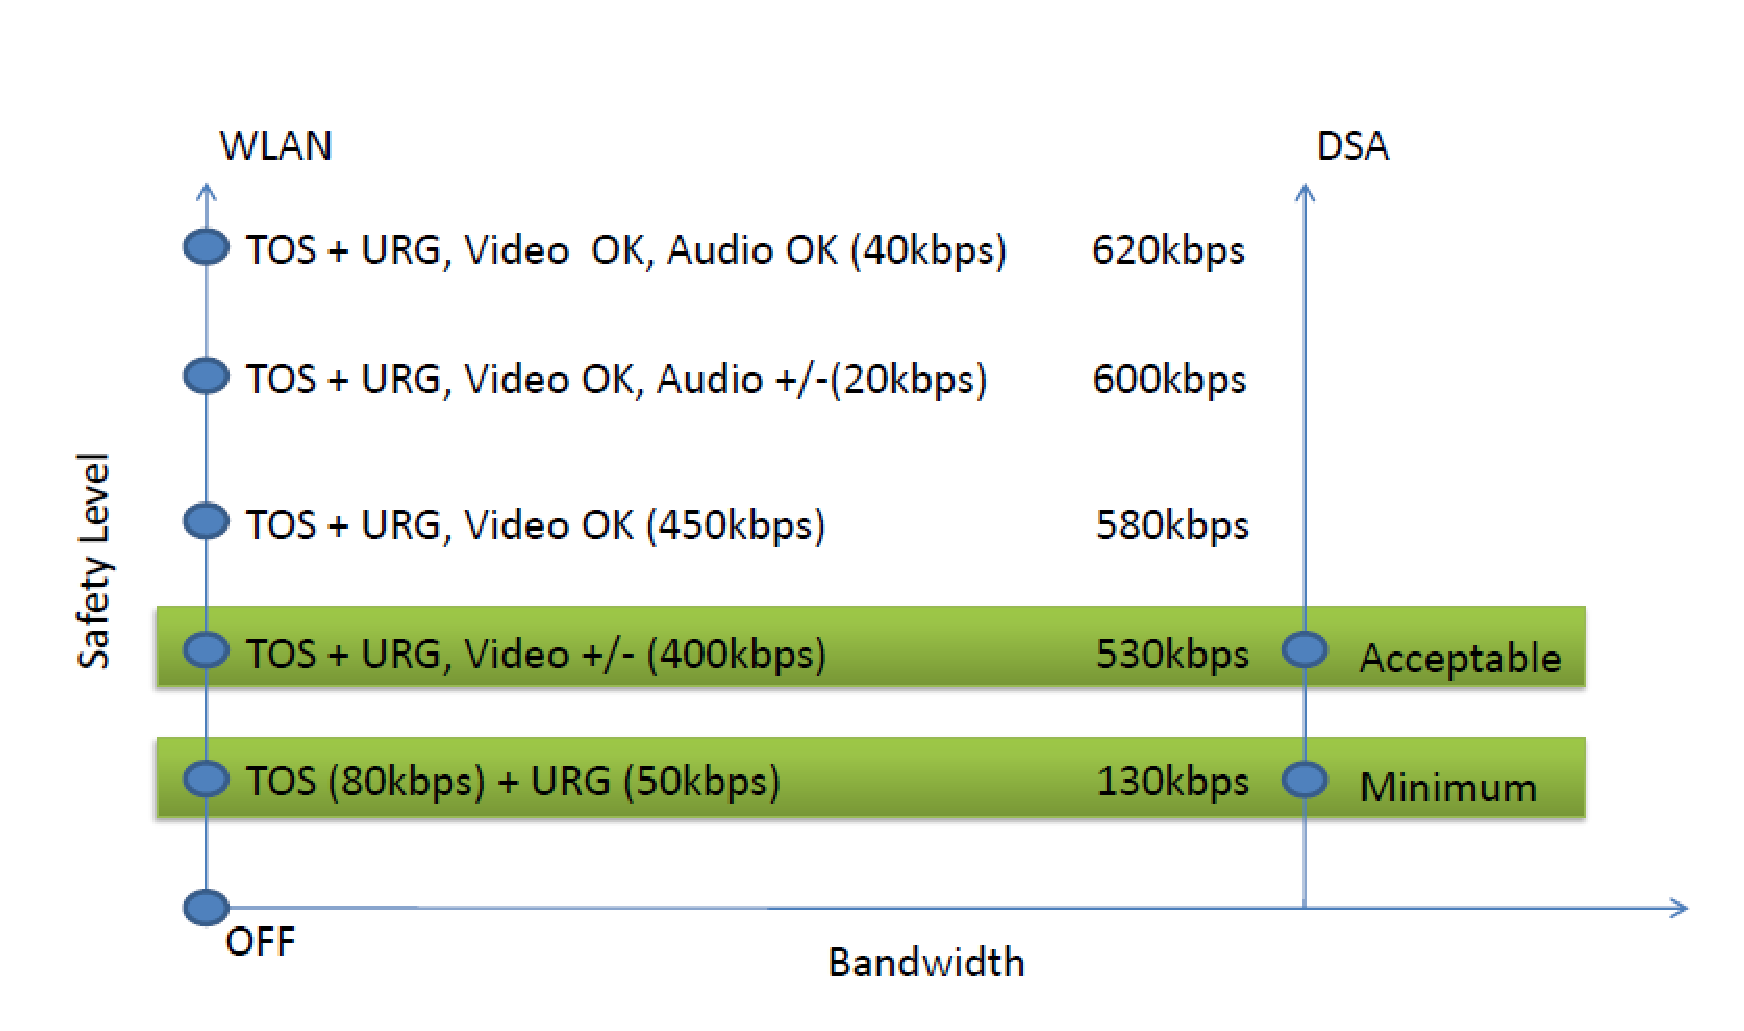
\includegraphics[width=1\columnwidth, scale=0.6]{dsaRoleResults}
\caption{DSA may work as a backup protocol in the event of a problem with the current WLAN protocols for traffic control.}
\label{fig:dsaRoleResults}
\end{figure}

\section{Results}
The results of the consumption of bandwith for each case is presented in Figures \ref{fig:expResults} a)- d).

From the analysis of these results and their effect on the controllability of the robot(s), it was concluded that the minimum amount of throughput necessary for the operation of a single mobile social robot is 130kbps, as can be seen in Figure \ref{fig:dsaRoleResults}.

This amounts for the total amount of telemetry sent from the robot to the operator (TOS, 80kbps) and the laser range finder data send to the operator (URG, 50kbps).
This minimum amount would at least allow an operator to know the current status of the robot and its location.
It would also enable the operator to move the robot, in a slow manner, to a safe location.

An minimum acceptable value for the safe teleoperation of a single mobile social robot is 530kbps.
This amount is the result of adding the previous 130kbps minimal required value and a slow, ``chopped'' video stream of 400kbps.

With a througput of 530kbps the operator may be able to observe the environment around the robot and move it to a safe location.
However, this amount of throughput would not allow for the operator to engage in a satisfactory interaction with a customer.
 

\end{document}
